% Emacs settings: -*-mode: latex; TeX-master: "manual.tex"; -*-

\begingroup                     % Make all definitions local.

%
% This was modified from risoe.sty, <2 Aug 95>
%
\catcode`\@=11
\def\@magscale#1{ scaled \magstep#1 }
\font\frtnbf = cmb10 \@magscale2
\font\twfvbf = cmbx10   \@magscale5 % extended bold
\def\maketitle{\par
 \begingroup
 \def\thefootnote{\fnsymbol{footnote}}
 \def\@makefnmark{\hbox to 0pt{$^{\@thefnmark}$\hss}}
 \if@twocolumn
 \twocolumn[\@maketitle]
 \else \newpage
 \global\@topnum\z@ \@maketitle \fi\thispagestyle{empty}\@thanks\newpage
 \endgroup
 \setcounter{footnote}{0}
 \let\maketitle\relax
 \let\@maketitle\relax
 \gdef\@thanks{}\gdef\@author{}\gdef\@title{}\let\thanks\relax}
\def\@maketitle{\newpage \baselineskip 30dd \mbox{}
 \marginpar{{\frtnbf \hfill \llap{\mbox{\reportnum \reportlan\qquad\qquad}}}}
 \par\noindent\mbox{
\includegraphics[height=1.5cm]{figures/risoe-logo.eps}\hspace{2mm}
\includegraphics[height=1.5cm]{figures/DTU_logo.ps}} \par
 \vskip 1.5cm
 {\twfvbf \noindent \@title \par} \vskip 20dd \baselineskip 16dd
 {\frtnbf\noindent\@author \par} 
 \vskip 0.5cm
 \begin{center}
     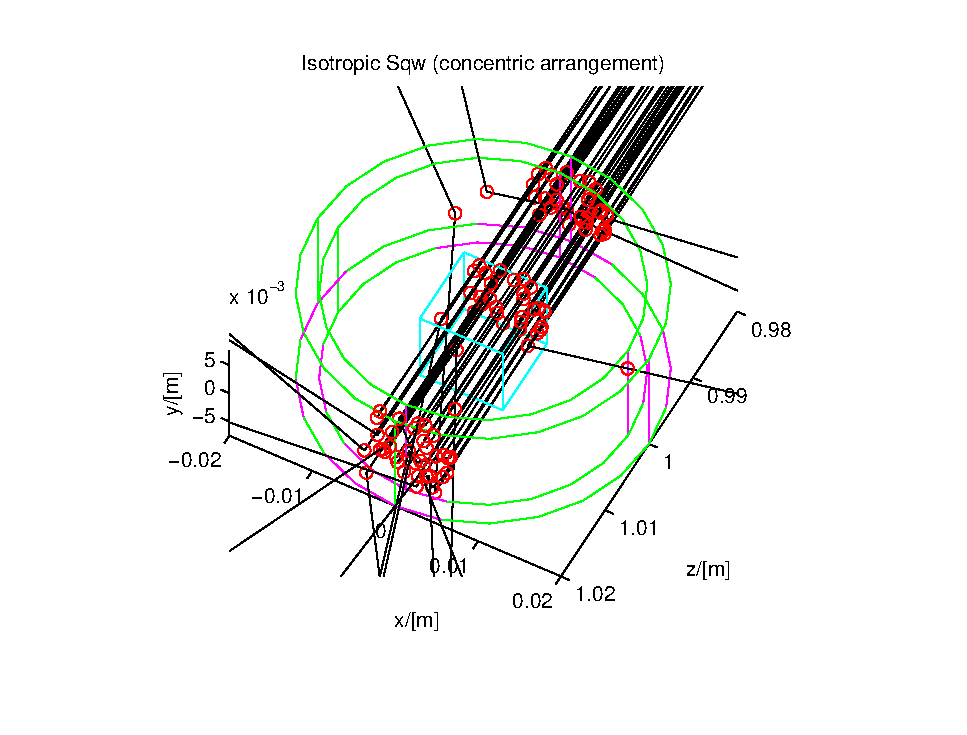
\includegraphics[width=\textwidth]{figures/sqw.eps}
   \end{center}
   \par \vfill \baselineskip 12dd
 \frtnbf\noindent Ris{\o} DTU, Roskilde, Denmark \par
 \vskip 4dd \noindent\ifcase\month\or
 January\or February\or March\or April\or May\or June\or
 July\or August\or September\or October\or November\or December\fi
 \space\number\year }

\let\reportlan=\relax
\def\month{5}                   % Released in November 2005
% Need to match front page line breaking.
\title{Component~Manual~for~\rlap{the}\\ % Avoid overfull message.
 Neutron~Ray-Tracing~Package\\
 \MCS, Version \version\ }
\author{Peter Kj\ae r Willendrup, Erik Knudsen, Kim Lefmann and\\Emmanuel Farhi}
\maketitle
\endgroup
